\documentclass{gemnumber} % Clase del Grupo Estudiantil de Matemática para el curso de Teoría de números.

\newcommand*{\colorboxed}{}
\def\colorboxed#1#{%
	\colorboxedAux{#1}%
}
\newcommand*{\colorboxedAux}[3]{%
	% #1: optional argument for color model
	% #2: color specification
	% #3: formula
	\begingroup
	\colorlet{cb@saved}{.}%
	\color#1{#2}%
	\boxed{%
		\color{cb@saved}%
		#3%
	}%
	\endgroup
}

%\usepackage[citestyle=numeric,style=numeric,backend=biber]{biblatex}
%\addbibresource{num.bib}
\DeclareMathOperator{\mcd}{mcd}
\newcommand{\MVAt}{{\usefont{U}{mvs}{m}{n}\symbol{`@}}} % Se prefiere no usar el paquete marvosym cuando esté cargada mathabx.
\renewcommand{\qedsymbol}{$\blacksquare$}
\newtheorem{definition}{Definición}[chapter] %chapter, section
\newtheorem{theorem}{Teorema}[chapter] %chapter section
\newtheorem{remark}{Observación}[chapter]
\newtheorem{conjecture}{Conjetura}
\theoremstyle{definition}
\pagestyle{empty} % Dentro de este archivo se encuentran los comandos, también puede agregar paquetes según su gusto.

\title{\Huge\bfseries\textcolor{DarkBlue}{Apuntes de clases de Teoría de números}}
\author{\LARGE\textcolor{DarkRed}{Grupo Estudiantil de Matemática}}
\date{\textcolor{DarkMagenta}{Actualizado a la fecha \today}}

\begin{document}

\maketitle

\chapter*{Prefacio}

Estos son los apuntes de clases de Teoría de números organizado por el \href{https://web.facebook.com/GEMFCUNI/}{Grupo Estudiantil de Matemática} durante los meses de enero y febrero del año 2018.

Muchas gracias al \href{http://imca.edu.pe/portal/index.php/es/}{Instituto de Matemática y Ciencias Afines} por brindarnos sus ambientes para llevar a cabo las clases.

Por favor, cualquier sugerencia o aviso de error escribir a {\href{mailto:gem@uni.edu.pe}{gem\MVAt uni.edu.pe}} o {\href{mailto:caznaranl@uni.pe}{caznaranl\MVAt uni.pe}}.

\begin{flushright}
	Carlos Aznarán
	
\end{flushright}

\begin{figure}[h]
	\begin{subfigure}[b]{.5\textwidth}
		\centering
		\captionsetup{justification=centering,margin=0.5cm}
		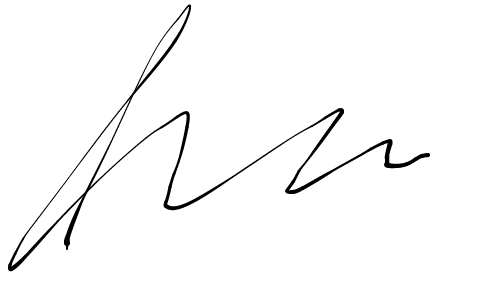
\includegraphics[height=4\baselineskip,width=.4\linewidth]{signature.png}
		\caption*{\textbf{Und. Jimmy Espinoza Palacios}\\Miembro del GEM\\Facultad de Ciencias}
	\end{subfigure}
	\begin{subfigure}[b]{.5\textwidth}
		\centering
		\captionsetup{justification=centering,margin=0.5cm}
		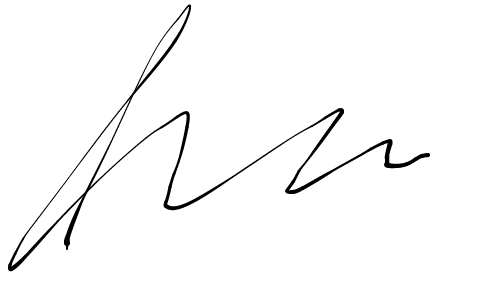
\includegraphics[height=4\baselineskip,width=.4\linewidth]{signature.png}
		\caption*{\textbf{Und. Bruno Goicochea Vilela}\\Presidente del GEM\\Facultad de Ciencias}
	\end{subfigure}
\end{figure}% Your signature
%El código fuente se puede encontrar en

\newpage

\renewcommand{\contentsname}{Tabla de contenido}

\tableofcontents

\chapter*{Un poco acerca de la historia de la \emph{Teoría de números}}

En el año 1912, durante el quinto 
\href{https://www.mathunion.org/organization/imu-history}{Congreso Internacional de Matemáticos}, el matemático alemán, en tal evento, \href{https://en.wikipedia.org/wiki/Edmund_Landau}{Edmund Landau} listó cuatro problemas básicos acerca de \emph{los números primos} que los calificó como \emph{inabarcable en el estado actual de las matemáticas} y en nuestros días es conocido como los \textbf{Problemas de Landau}. Ellos son los siguientes:
\begin{enumerate}
	\item Conjetura de Goldbach\footnote{Helfgott probó la conjetura débil en el año 2013.}
	\item Conjetura de los primos gemelos.
	\item Conjetura de Legendre.
	\item ¿Existen infinitos números primos de la forma $n^{2}+1$?
\end{enumerate}

Ninguno de los cuatro problemas han sido resultados a la fecha de la edición de los apuntes.

La teoría de números tal como se conoce en la actualidad inició desde Gauss. En el año 2013, el matemático peruano Harald Andrés Helfgott demostró la \emph{Conjetura débil (o ternaria) de Goldbach}
%https://www.gaussianos.com/harald-andres-helfgott-nos-habla-sobre-su-demostracion-de-la-conjetura-debil-de-goldbach/
\section{Harald Andrés Helfgott}
\begin{conjecture}{Goldbach}
Todo número impar mayor que cinco es la suma de tres números primos.
\end{conjecture}
\emph{Leonhard Euler}, uno de los más grandes matemáticos del siglo XVIII, y de todas las épocas, y su amigo cercano \emph{Christian Goldbach}, quien tenía grandes conocimientos tanto en la ciencia como en las humanidades, mantuvo una regular y copiosa correspondencia. Goldbach hizo una conjetura acerca de los números primos, y Euler rápidamente redujo a la siguiente conjetura, el cual, dijo, Goldbach ya le había dicho: cada entero positivo puede escribirse a lo más, como la suma de tres números primos.

%En el año X, Terence Tao probó para el caso como la suma de cinco números primos.

Ahora, podríamos decir que ``cada entero mayor que cinco'', ya que no consideramos a 1 como un número primo. Es más, en la actualidad la conjetura se divide en dos casos: la \emph{conjetura débil o ternaria de Goldbach} establece que cada entero impar mayor que cinco se puede escribir como la suma de tres primos y la \emph{conjetura fuerte o binaria de Goldbach} establece que cada entero par mayor que 2 se puede escribir como la suma de dos primos. Como indican sus nombres, la conjetura fuerte implica la débil (fácilmente: reste 3 al número impar $n$, luego exprese $n-3$ como la suma de dos números primos).
%https://valuevar.wordpress.com/2013/07/02/the-ternary-goldbach-conjecture/
%http://libgen.io/search.php?&req=History+of+the+theory+of+numbers+Dickson&phrase=1&view=simple&column=def&sort=year&sortmode=DESC
%Cayley y Sylvester trabajaron en la conjetura de Goldbach.
%Citar el libro de Escalante sobre las figuras.
%Grandes matemáticos de Temple Bell.

La Olimpiada Internacional de Matemática (IMO) es la Olimpiada científica más grande, más antigua y más prestigiosa para estudiantes de secundaria. La historia de la IMO se remonta a 1959, cuando la primera edición se celebró en Rumanía y participaron siete países: Rumanía, Hungría, Bulgaria, Polonia, Checoslovaquia, Alemania Oriental y la URSS. Desde entonces, el evento se ha celebrado todos los años (excepto 1980) en un país diferente. Actualmente, participan más de 100 países de los 5 continentes. Cada país puede enviar un equipo de hasta seis estudiantes secundarios o individuos que no hayan ingresado a la Universidad o su equivalente,

as of the date of celebration of the Olympiad, plus one team leader, one deputy leader, and observers if desired.

During the competition, contestants have to solve, individually, two contest papers on two consecutive days, with three problems each day. Each problem is worth seven points. Gold, silver, and bronze medals are awarded in the ratio of 1:2:3 according to the overall results — half of the contestants receive a medal. In order to encourage as many students as possible to solve complete problems, certificates of honorable mention are awarded to students (not receiving a medal) who obtained 7 points for at least one problem.

\begin{figure}[H]
	\centering
	\def\svgwidth{7cm}
	\input{imo2018.pdf_tex}	
\end{figure}

 a partir de la fecha de celebración de la Olimpiada, más un líder de equipo, un líder adjunto y observadores si así lo desean. Durante la competencia, los concursantes deben resolver, individualmente, dos documentos del concurso en dos días consecutivos, con tres problemas cada día. Cada problema vale siete puntos. Las medallas de oro, plata y bronce se otorgan en una proporción de 1: 2: 3 de acuerdo con los resultados generales: la mitad de los concursantes reciben una medalla. Con el fin de alentar a tantos estudiantes como sea posible para resolver problemas completos, se otorgan certificados de mención honorífica a los estudiantes (que no reciben una medalla) que obtuvieron 7 puntos por al menos un problema.


\chapter{Introducción} %Fecha: 11 de enero del 2018.

\begin{enumerate}[font={\bfseries},label={\roman*.}]

\item\label{pr:1} \emph{Principio de inducción matemática}
	
Sea $\mathcal{P}$ un conjunto de números naturales tal que

\begin{enumerate}
	\item $1\in\mathcal{P}$.
	\item Si $n\in\mathcal{P}\implies n+1\in\mathcal{P}$.
\end{enumerate}

$\therefore \boxed{\mathcal{P}=\mathbb{N}}$.

\item\label{pr:2} \emph{Principio del buen orden}

Si $\mathcal{A}$ es un conjunto no vacío de $\mathbb{N}$, entonces \emph{$\mathcal{A}$ posee un elemento mínimo}.

\end{enumerate}

\section{Divisibilidad}

\begin{definition}\label{def:1.1}

Sean $d$ y $n$ dos números enteros, se denotará

\[\boxed{d\text{ divide a }n\iff\text{ existe }c\in\mathbb{Z}\text{ tal que }n=c\cdot n}\]
como $a\divides n$.

\noindent
Si $d$ no divide a $n$, es decir, si $\forall c\in\mathbb{Z}\colon n\neq c\cdot d$, se denotará como $d\notdivides n$.

\end{definition}

\subsection{Propiedades de la operación $|$}

\begin{enumerate}[font={\bfseries},label={\arabic*)}]

\item\label{prop:1} $n\divides n$ para cualquier $n\in\mathbb{N}$ (Reflexividad).

\item\label{prop:2} Si $d\divides n$ y $n\divides m$, entonces $d\divides m$. (Transitividad).

\item\label{prop:3} Si $d\divides n$ y $d\divides m$, entonces $d\divides an+bm$ $\forall a,b\in\mathbb{Z}$.

\item\label{prop:4} Si $d\divides n$, entonces $ad\divides an$.

\item\label{prop:5} Si $ad\divides an$ con $a\neq0$, entonces $d\divides n$.

\item\label{prop:6} $1\divides n$ para cualquier $n\in\mathbb{N}$.

\item\label{prop:7} $n\divides 0$ para cualquier $n\in\mathbb{N}$.

\item\label{prop:8} Si $0\divides n$, entonces $n=0$.

\item\label{prop:9} Si $d\divides n$ y $n\neq0$, entonces $|d|\leq|n|$.

\item\label{prop:10} Si $d\divides n$ y $n\divides d$, entonces $|d|=|n|$.

\item\label{prop:11} Si $d\divides n$ con $d\neq0$, entonces $\left(\frac{n}{d}\right)\divides n$.

\end{enumerate}

\section{Máximo común divisor}

\begin{definition}\label{def:1.2}

Sean $a$, $b$ y $d$ números enteros. Si $d\divides a$ y $d\divides b$, entonces $d$ es un divisor común de $a$ y $b$.

\end{definition}

\begin{theorem}\label{teo:1.1}

Dados los números enteros $a$ y $b$, existe un divisor común $d$ de $a$ y $b$ de la forma $d=ax+by$ para cualesquiera $x,y\in\mathbb{Z}$.

\begin{proof}[Prueba:]
Por inducción matemática en $K=|a|+|b|$.
 
Si $K=0$, entonces $a=b=0$, esto es, $d=0\cdot a+0\cdot b$. \checkmark
	 
\noindent
Supongamos que se cumple para $K=0,1,\ldots,n-1$. (Hipótesis de inducción matemática).
	 
Demostraremos para $\boxed{K=n=|a|+|b|}$.
	 
\noindent
Sin pérdida de generalidad, suponga que $|a|\geq|b|$. Así, si $|b|=0$, entonces $b=0$ y $|a|=n\implies d=n=(1)(\pm1)+0\cdot b$.
	 
Si $|b|\geq1$, entonces para los números $|a|-|b|$ y $|b|$ se cumple la hipótesis:

\[\underbrace{|a|-|b|}_{\displaystyle\geq0}+|b|=|a|-\cancel{|b|}+\bcancel{|b|}=|a|<|a|+|b|=n.\]

Existe $d\in\mathbb{Z}$, $d\divides |a|-|b|$ y $d\divides |b|$. Además:

\begin{align*}
	d&=\left(|a|-|b|\right)x^{\prime}+|b|y^{\prime}&\forall x^{\prime},y^{\prime}\in\mathbb{Z}\\
	d&=|a|\underbrace{x^{\prime}}_{\displaystyle x^{\prime\prime}}+|b|\underbrace{y^{\prime}}_{\displaystyle y^{\prime\prime}}&\\
	d&=\underbrace{|a|}_{a,-a}x^{\prime\prime}+\underbrace{|b|}_{b,-b}y^{\prime\prime}&\\
	d&=a\underbrace{x^{\prime\prime}}_{\pm x^{\prime}}+b\underbrace{y^{\prime\prime}}_{\pm y^{\prime}}&
\end{align*}

\noindent
Pero $d\divides |a|$ y $d\divides |b|$, así $d\divides |a|-|b|$.

\noindent
$\therefore$ Esto cumple la condición.
\end{proof}

\end{theorem}

\begin{theorem}\label{teo:1.2}
Sean $a$ y $b$ números enteros, existe solo un número $d\in\mathbb{Z}$ tal que

\begin{enumerate}[font={\bfseries},label={\arabic*)}]

\item\label{teo1.2:1} $d\geq0$.

\item\label{teo1.2:2} $d\divides a$ y $d\divides b$.

\item\label{teo1.2:3} Si $e\divides a$ y $e\divides b$, entonces $e\divides d$ para cualquier $e\in\mathbb{Z}$.

\end{enumerate}

\begin{proof}[Prueba:]
Por la definición~\ref{def:1.2} y por el teorema~\ref{teo:1.1}, existe un $d$ con las siguientes propiedades:
\begin{multicols}{3}
$d\divides a$

$d\divides b$

$d=ax+by$
\end{multicols}

\noindent
Es claro que $-d$ también cumple esto. Elegimos $|d|=ax^{\prime}+by^{\prime}$ que cumpla \ref{teo1.2:1} y \ref{teo1.2:2}.

\noindent
Si $e\divides a$ y $e\divides b$, entonces de la propiedad~\ref{prop:3} $e\divides ax^{\prime}+by^{\prime}=|d|$.
	
\noindent
Así, $e\divides |d|$, en consecuencia $e\divides d$ y $|d|$ satisface~\ref*{teo1.2:3}.
	
\noindent
Si existiese un $d^{\prime}$ que cumpla \ref{teo1.2:1}, \ref{teo1.2:2} y \ref{teo1.2:3}, entonces de la afirmación \ref{teo1.2:3}:

\begin{equation}\label{eq:1.1}
d\divides a\text{ y }d\divides b\implies d\divides d^{\prime}.
\end{equation}
	
\noindent
De forma similar:
\begin{equation}\label{eq:1.2}
d^{\prime}\divides a\text{ y }d^{\prime}\divides b\implies d^{\prime}\divides d.
\end{equation}

\noindent
Pero de~\eqref{eq:1.1} y \eqref{eq:1.2} junto con la propiedad~\ref{prop:10} se obtiene que $\boxed{d=d^{\prime}}$.
\end{proof}

\end{theorem}

\begin{definition}
Este número $d$ es llamado máximo común divisor de $a$ y $b$ y se denota como $\mcd(a,b)$ o $(a,b)$.
\end{definition}

\begin{remark}
Si el $\mcd(a,b)=1$, entonces $a$ y $b$ son llamados coprimos, primos entre sí (PESI) o primos relativos.
\end{remark}

\subsection{Algunas propiedades del máximo común divisor}

\begin{enumerate}[font={\bfseries},label={\arabic*)}]

\item $(a,b)=(b,a)$.

\item $(a,(b,c))=((a,b),c)$.

\item $(ac,bc)=|c|(a,b)$.

\item $(a,1)=(1,a)=1$.

\item $(a,0)=(0,a)=|a|$.
\end{enumerate}

\begin{theorem}

Si $a\divides bc$ y si $(a,b)=1$, entonces $a\divides c$.
\begin{proof}
Como $(a,b)=1$, entonces existen $\tilde{x},\tilde{y}\in\mathbb{Z}$ de modo que

\begin{equation}\label{eq:1.3}
1=a\tilde{x}+b\tilde{y}
\end{equation}

\noindent
Pero si multiplicamos~\eqref{eq:1.3} por $c$ resulta
\begin{equation}
c=a(c\tilde{x})+b(c\tilde{y})
\end{equation}
Así, $a\divides cx$ y $a\divides cy$ (explicar).

\end{proof}

\end{theorem}

\section{Números primos}

\begin{definition}

El número $n\in\mathbb{N}$ es llamado número primo si sus divisores positivos son 1 y $n$. Cuando $n$ no es primo, será llamado número compuesto. 

\end{definition}

\begin{theorem}
Cada natural $n>$ 1 o es primo o producto de números primos.

\begin{proof}[Prueba:]
Por inducción sobre $n$.

Para $n=2$ \checkmark

Supongamos que se cumple para $n=2,3,\ldots,k-1$.

Demostraremos para $n=k$.

\begin{enumerate}[font={\bfseries},label={*)}]

\item Si $k$ es un número primo.

\item Si $k$ no es un número primo, entonces $k$ tiene por lo menos un divisor $d>1$, por lo que $k=d\cdot c$ con $1<c<k$ y $1<d<k$.

\end{enumerate}

\noindent
Se cumple la hipótesis para $c$ y $d$, entonces $c$ y $d$ son primos o productos de primos.

\begin{align*}
c&=p_1p_2\cdots p_k&(p_i\colon\text{primo}, k\geq1).\\
d&=q_1q_2\cdots q_m&(q_i\colon\text{primo}, m\geq1).
\end{align*}

\noindent
Así, $n=c\cdot d=p_1p_2\cdots p_kq_1q_2\cdots q_m$ (se cumple la inducción).
\end{proof}
\end{theorem}

\begin{theorem}
Existen infinitos números primos.

\begin{proof}[Prueba:]

Supongamos que $\boxed{\mathbb{P}=p_1p_2\cdots p_k}$ es el conjunto  de todos los números primos que existen. Definimos:
\[N=p_1p_2\cdots p_k+1\]
¿Qué tipo de número es $N$, es un primo o uno compuesto?

\noindent
Claro está que $N$ es mayor que $p_i,\forall i=1,\cdots k$.

$N=p_1p_2\cdots p_k+1=q_1q_2\cdots q_t$.

\[\begin{array}{l@{\quad}cr@{}l}
&& q_i & {}\divides p_1p_2\cdots p_k+1 \\
&& q_i & {}\divides p_1p_2\cdots p_k \\ \cline{2-4}
&& q_i & {}\divides 1\quad(\implies\impliedby)
\end{array}\ (-)\]
$\therefore$ Existen infinitos números primos. %(¿numerable?)
\end{proof}

\end{theorem}

\begin{theorem}
Si $p$ es un número primo y $p\notdivides a$, entonces $(p,a)=1$.

\begin{proof}

Sea $d$ el máximo común divisor de $p$ y $a$ (ya que el teorema~\ref{teo:1.1} nos asegura su existencia), $d=(p,a)$, entonces

\[d\divides p\quad\text{y}\quad d\divides a.\]

\end{proof}

\end{theorem}

\begin{theorem}

Sea $p$ un número primo. Si $p\divides ab$, entonces $p\divides a$ o $p\divides b$.

\begin{proof}[Demostración:]
Supongamos que $p\notdivides a$ ($p\divides a$ \checkmark), entonces $(p,a)=1$, en consecuencia, $p\divides ab$.

\[\colorboxed{DarkRed}{a\divides bc\quad\text{y}\quad(a,b)=1\implies a\divides c.}\]

\noindent
$\therefore p\divides b$.
\end{proof}

\end{theorem}

%Generalización: Si $p\divides a_1a_2\cdots a_n\implies p\divides a_1,\ldots, p\divides a_n$. Donde $p$ es un número primo.
\begin{theorem}

Cada entero $n>1$ se representa de forma única como producto de primos no necesariamente distintos, sin importar el orden.

\begin{proof}[Prueba:]

Por inducción en $n$. Cuando $n=2$ (se cumple: 2,3,\ldots,n-1.)
$n=p_1p_2\cdots,p_s=q_1q_2\cdots q_t$ ($s=t$).
$(s,t\geq 1)$

$p_1\divides q_1q_2\cdots q_t\implies p_1\divides q_1\implies p_1=q_1$.
\end{proof}

\end{theorem}

\begin{remark}

Si se desea representar a $n$ como producto de primos distintos (donde cabe la posibilidad en que se repitan algún número primo), podemos escribir:
\[n={p}^{a_1}_{1}{p}^{a_2}_{2}\cdots{p}^{a_k}_{k}=\prod_{i=1}^{k}{p}^{a_i}_{i}\]

\end{remark}

\begin{theorem}

Si $\displaystyle n=\prod_{i=1}^{r}{p}^{a_i}_{i}$, entonces un divisor de $n$ tiene la forma
\[\prod_{i=1}^{r}={p}^{c_i}_{i},\quad0\leq c_i\leq a_i.\]

\end{theorem}

\begin{remark}

Sea la sucesión de números primos
\[p_1=2, p_2=3, p_3=5, \ldots,\]
entonces $\displaystyle n=\prod_{i=1}^{\infty}{p}^{a_i}_{i},\, a_i\geq0$.

\end{remark}

\begin{theorem}

Sean $\displaystyle a=\prod_{i=1}^{\infty}{p}^{a_i}_{i}$ y $\displaystyle b=\prod_{i=1}^{\infty}{p}^{b_i}_{i}$, entonces el máximo común divisor de $a$ y $b$ es

\[(a,b)=\displaystyle\prod_{i=1}^{\infty}{p}^{c_i}_{i}\geq0\text{, donde }c_i=\min\{a_i,b_i\}\leq a_i,b_i.\]

\begin{proof}[Demostración:]

\begin{enumerate}[font={\bfseries},label={*)}]

\item $\displaystyle\prod_{i=1}^{\infty}{p}^{c_i}_{i}\divides a\quad\wedge\quad\prod_{i=1}^{\infty}{p}^{c_i}_{i}\divides b$.

\item $e\divides a\quad\wedge\quad e\divides b, e=\displaystyle\prod_{i=1}^{\infty}{p}^{e_i}_{i}$.

\end{enumerate}

\noindent
Pero, $e_i\leq a_i$ y $e_i\leq b_i$,

\[\implies e_i\leq\min\{a_i,b_i\}=c_i.\]

\[e=\prod_{i=1}^{\infty}{p}^{e_i}_{i}\divides\prod_{i=1}^{\infty}{p}^{c_i}_{i}=(a,b).\]
\end{proof}

\end{theorem}

\begin{theorem}

Sean $a$ y $b$ números enteros con $b>0$, entonces existen únicos $q,r\in\mathbb{Z}$ tal que:

\[a=bq+r,\quad0\leq r<b.\]

\noindent
Además, $r=0\iff b\divides a$.

\begin{proof}[Demostración:]
Fijando $\underline{b}$ y por inducción en $a\in\mathbb{N}$. Si $a=0$, entonces $a=b\cdot0+0$. \checkmark

\noindent
Supongamos que se cumple para $a=0,1,\ldots,k-1$.

\noindent
Para $a=k$. $k-1=b\cdot q^{\prime}+r^{\prime}$, $0\leq r^{\prime}<b$.
\[\longrightarrow k=bq^{\prime}+(r^{\prime}+1).\quad1\leq r^{\prime}+1<b+1.\]

\begin{enumerate}[font={\bfseries},label={$\bullet$)}]

\item Si $1\leq r^{\prime}+1<b$ \checkmark

\item Si $r^{\prime}+1=b\rightarrow r^{\prime}=b-1\implies$

\end{enumerate}
\end{proof}

\end{theorem}

\chapter{Ejercicios}
\section{Lista N$^{\circ}1$}
\begin{enumerate}[font={\bfseries},label={\arabic*.}]
\item Un número racional $a/b$ con $(a,b)=1$ se llama \emph{fracción reducida}. Si la suma de dos fracciones reducidas es un entero, es decir, si $(a/b)+(c/d)=n$. Demostrar que entonces $|b|=|d|$.

\item Si $(a,b)=1$, entonces $(a+b,a-b)$ o es 1 o es 2.

\item Si $(a,b)=1$, entonces $(a+b,a^{2}-ab+b^{2})$ o es 1 o es 3.

\item Si $(a,b)=1$, entonces $(a^{n},b^{k})=1$ para todo $n\geq1, k\geq1$.

\item Un entero se llama \emph{sin cuadrados} si no es divisible por el cuadrado de ningún primo. Probar que, para cada $n\geq1$, existen $a>0$ y $b>0$, unívocamente determinados, tales que $n=a^{2}b$, en donde $b$ es sin cuadrados.

\item Probar que $\dfrac{21n+4}{14n+3}$ es irreducible para todo número natural $n$.

\item Sean $\{a,b,x,y\}\subset\mathbb{N}$. Si $(a,b)=1$ y $ab=c^{n}$, probar que $a=x^{n}$ y $b=y^{n}$ para algunos $x,y$ enteros positivos.

\item Hallar $\left(a^{2^{m}}+1,a^{2^{n}}+1\right)$ en función de $a$.

\item Sean $\{a,b,x,y\}\subset\mathbb{N}$. Si $(a,b)=1$ y $x^{a}=y^{b}$ entonces probar que $x=n^{b}$ e $y=n^{a}$ para algún entero positivo.

\item Si $\{a,m,n\}\subset\mathbb{N}$ con $a>1$, probar que $\left(a^{m}-1,a^{n}-1\right)=a^{(m,n)}-1$.

\item Sea $n$ un entero positivo y sea $S$ un conjunto de enteros positivos menores o iguales a $2n$ tal que si $a$ y $b$ están en $S$ y $a$ y $b$ son diferentes, entonces $a$ no divide a $b$. Hallar el máximo número de elementos de $S$.

\item Hallar todos los pares de enteros positivos $(a,b)$ tales que $a\divides b+1$ y $b\divides a+1$.

\item Hallar todos los pares de enteros positivos $(a,b)$ tales que $a\divides8b+1$ y $b\divides8a+1$.

\item Halle todos los números enteros positivos $n$ tales que el conjunto $\{n,n+1,n+2,n+3,n+4,n+5\}$ puede ser particionado en dos subconjuntos de modo que el producto de los números en cada subconjunto sea igual.

\item Sea $m$ y $n$ números enteros tales que:
\[\frac{m}{n}=1-\frac{1}{2}+\frac{1}{3}-\frac{1}{4}+\cdots-\frac{1}{1318}+\frac{1}{1319}\]

Probar que $m$ es divisible por 1979. Ayuda: 1979 es un número primo.
\end{enumerate}

\section{Solución de la lista N$^{\circ}$1}

\begin{enumerate}[font={\bfseries},label={\arabic*.}]
\item
	\begin{enumerate}[font={\bfseries}]
	\item Dado $n=\dfrac{ad+bc}{bd}$, con $b$ y $d$ que dividen a $ad+bc$. Esto significa que $b\divides bc$ y $d\divides bc$, pero $\mcd(a,b)=\mcd(c,d)=1$. se tiene que $b\divides b$ y $d\divides b$. Por lo tanto, $|b|=|d|$.
	
	\item Sea $k\in\mathbb{Z}$ y $k=\dfrac{a}{b}+\dfrac{c}{d}$, entonces $\dfrac{c}{d}=k-\dfrac{a}{b}=\dfrac{ck-a}{b}$.
	
	Supongamos por contradicción que $\mcd(kb-a,b)\neq1$. Además, si $\mcd(kb-a,b)=n$, entonces $n\divides (kb-a)$ y  $n\divides b$.
		
	\[kb-a=n\ell_1\quad\wedge\quad b=n\ell_2\]
	\[k(n\ell_2)-a=n\ell_1\]
	\[n(k\ell_2-\ell_1)=a\]
	Pero de la última ecuación, se infiere que $n\divides a$ y $n\divides b$, lo cual es una contradicción.
	\end{enumerate}
	
	\item Si el $\mcd(a,b)=1$ y el $\mcd(a+b,a-b)=d$, entonces:
	
	\begin{align*}
	d\divides a+b\;&\wedge\; d\divides a-b&\implies d&\divides (a+b)+(a-b)\;&\wedge\; d&\divides (a+b)-(a-b)&\\
	d\divides a+b\;&\wedge\; d\divides a-b&\implies d&\divides 2a\;&\wedge\; d&\divides 2b&
	\end{align*}
	Por lo tanto $d\divides \mcd(2a,2b)\implies d\divides 2\mcd(a,b)\implies d\divides 2$, así, $d=1\vee2$.
	
	\item Si el $\mcd(a,b)=1$ y el $\mcd(a+b,a^{2}-ab+b^{2})=d$, entonces:
	
	\begin{align*}
	d\divides a+b\;&\wedge\; d\divides a^{2}-ab+b^{2}&\implies d&\divides {(a+b)}^{2}\;&\\
	d\divides a+b\;&\wedge\; d\divides a^{2}-ab+b^{2}&\implies d&\divides a^{2}+2ab+b^{2}\;&\\
	d\divides a+b\;&\wedge\; d\divides a^{2}-ab+b^{2}&\implies d&\divides
	\cancel{a^{2}}+2ab+\cancel{b^{2}}-(\bcancel{a^{2}}-ab+\bcancel{b^{2}})\;&&\\
	d\divides a+b\;&\wedge\; d\divides a^{2}-ab+b^{2}&\implies d&\divides3ab
	&
	\end{align*}
	Por lo tanto, $d\divides 3a(a+b)\implies d\divides 3a^{2}+3ab$. De esto, $d\divides 3a^{2}$ y $d\divides 3ab$.
	
	\[d\divides\mcd(3a^{2},3ab)\implies d\divides|3a|\cdot\mcd(a,b)\implies d\divides 3a.\]
	
	Como $d\divides a+b\implies d\divides 3a+3b\implies d\divides 3b$. %pues d divide a 3a
	$d\divides\mcd(3a,3b)\implies d\divides 3\underbrace{\mcd(a,b)}_{\displaystyle1}\implies d\divides 3$. Así, $d=1\vee3$.
	
	\item Si el $\mcd(a,b)=1$ y el $\mcd(a^{n},b^{k})=d>1$, entonces $d\divides a^{n}$ y $d\divides b^{k}$. Sea $p$ un número primo de modo que $p\divides d$. Así:
	\begin{align*}
	p\divides a^{n}\;\wedge\;p\divides b^{k}\implies p\divides a\;\wedge\; p\divides b\implies p\divides\underbrace{\mcd(a,b)}_{\displaystyle1}
	\end{align*}
	¡Un número primo divide a 1! $(\implies\impliedby)$. $\therefore d=1$.
	
	\item Sea el conjunto $\mathbb{N}=\mathcal{A}\bigcup\mathcal{B}$, donde $\mathcal{A}\coloneq\{n\in\mathbb{N}\mid n\text{ es libre de cuadrados} \}$ y $\mathcal{B}\coloneq\mathcal{A}^{\complement}$.
	
	Para el caso 1: Sea $\gamma=1^{2}\cdot\gamma$, si $\gamma\in\mathcal{A}$.
	
	Sea $\theta\in\mathcal{B}$, entonces $\exists z^{2}\ni\theta=z^{2}\cdot\tau$.
	
	Supongamos que $\tau$ no es libre de cuadrados:
	\[\tau=n^{2}\cdot m \checkmark\]
	Al reemplazar resulta:
	\[\theta=z^{2}n^{2}m=(z\cdot n)^{2}\cdot m(\implies\impliedby)\]
	
	\item Por contradicción y combinación lineal
	\[\mcd(a,b)=1\;\text{y}\;a\cdot b=c^{n}\]
	donde $a$ y $b$ tienen las siguiente forma:
	\[a={p}^{\alpha_1}_{1}{p}^{\alpha_2}_{2}\cdots{p}^{\alpha_k}_{k}\quad\text{y}\quad b={q}^{\beta_1}_{1}{q}^{\beta_2}_{2}\cdots{q}^{\beta_\ell}_{\ell}.\]
	¡Recuerde que a y b no tiene factores comunes!
	Así, multiplicando $a$ y $b$:
	\[
	a\cdot b={p}^{\alpha_1}_{1}{p}^{\alpha_2}_{2}\cdots{p}^{\alpha_k}_{k}\cdot{q}^{\beta_1}_{1}{q}^{\beta_2}_{2}\cdots{q}^{\beta_\ell}_{\ell}=c^{n},
	\]
	donde
	\[c={p}^{\theta_1}_{1}{p}^{\theta_2}_{2}\cdots{p}^{\theta_k}_{k}\cdot{q}^{\phi_1}_{1}{q}^{\phi_2}_{2}\cdots{q}^{\phi_\ell}_{\ell}\]
	\[c^{n}={p}^{\theta_1\cdot n}_{1}{p}^{\theta_2\cdot n}_{2}\cdots{p}^{\theta_k\cdot n}_{k}\cdot{q}^{\phi_1\cdot n}_{1}{q}^{\phi_2\cdot n}_{2}\cdots{q}^{\phi_\ell\cdot n}_{\ell}\]
	
	Por comparación obtenemos las siguientes igualdades:
	\[
	\alpha_1=\theta_1\cdot n,\;\alpha_2=\theta_2\cdot n,\;\cdots,\alpha_k=\theta_k\cdot n.%Tratar de reproducirlo con un foreach con Tikz.
	\]
	\[
	\beta_1=\phi_1\cdot n,\;\beta_2=\phi_2\cdot n,\;\cdots,\beta_\ell=\phi_\ell\cdot n.
	\]
	Así, $a={\left(\underbrace{{p}^{\theta_1}_{1}{p}^{\theta_2}_{2}\cdots{p}^{\theta_k}_{k}}_{\displaystyle x}\right)}^{n}$ y $b={\left(\underbrace{{q}^{\phi_1}_{1}{q}^{\phi_2}_{2}\cdots{q}^{\phi_\ell}_{\ell}}_{\displaystyle y}\right)}^{n}$.
	
	\item Sea $g=\mcd(\mathfrak{a}^{2^{m}}+1,\mathfrak{a}^{2^{n}}+1)$. Se define la aplicación $f_{\mathfrak{a}}$ con la siguiente regla de correspondencia como sigue:
	\[\begin{aligned}
	f_{\mathfrak{a}}\colon\mathbb{N}&\longrightarrow\mathbb{N}\\
	k&\longmapsto\mathfrak{a}^{2^{k}}+1
	\end{aligned}\]
	Así, con la notación apropiada, $g$ queda expresada como $\mcd\left(f_{\mathfrak{a}}(m),f_{\mathfrak{a}}(n)\right)$. Además $g\divides f_{\mathfrak{a}}(m)$ y $g\divides f_{\mathfrak{a}}(n)$.
	
	\begin{enumerate}
		\item Para el caso en que $m>n$:
		
		Ahora, calculemos:
		
		\begin{flalign*}
		f_{\mathfrak{a}}(m)-2
		&=\mathfrak{a}^{2^{m}}+1-2=\mathfrak{a}^{2^{m}}-1&\\
		&=\left(\mathfrak{a}^{2^{n}}\right)^{2^{m-n}}-1&\\
		&=\underbrace{\left(\mathfrak{a}^{2^{n}}+1\right)}_{\displaystyle f_{\mathfrak{a}}(n)}\left(\mathfrak{a}^{2^{(m-n-1)}}-1\right)&
		\end{flalign*}
		
		Así que $f_{\mathfrak{a}}(n)\divides f_{\mathfrak{a}}(m)-2$. Pero, como $g\divides f_{\mathfrak{a}}(n)\implies g\divides f_{\mathfrak{a}}(m)-2$
		
		\item Para el caso en que $m=n$:
		
		\item Para el caso en que $m<n$:
	\end{enumerate}
	
	\item Si el $\mcd(a,b)=1$ y los números $a$ y $b$ tiene la siguiente representación:
	\[a={p}^{\theta_1}_{1}{p}^{\theta_2}_{2}\cdots{p}^{\theta_k}_{k}=\prod_{i=1}^{k}{p_i}^{\alpha_i}\]
	\[b={q}^{\beta_1}_{1}{q}^{\beta_2}_{2}\cdots{q}^{\beta_\ell}_{\ell}=\prod_{i=1}^{\ell}{q_i}^{\beta_i}\]
	
	Pero $x^{a}=$
\end{enumerate}

\documentclass[oneside]{memoir}
\usepackage[utf8x]{inputenc}
\usepackage[spanish]{babel}
\spanishdatedel
\usepackage{amsfonts}
\usepackage{amsthm,mathabx}
\newtheorem{definition}{Definición}
\newtheorem{theorem}{Teorema}
\title{Teoría de números enteros}
\author{Oromion}
\begin{document}
\maketitle
\chapter{Divisibilidad}

\begin{definition}
Un entero $b$ es divisible por un entero $a$, no cero, si existe un entero $x$ tal que $b=ax$ y se escribe a $a\divides b$. En el caso en que $b$ no sea divisible por a se escribe $a\notdivides b$.
\end{definition}

\begin{theorem}
\noindent
Sean $\{a,b,c,x,y\}\subset\mathbb{Z}$, las siguientes proposiciones son verdaderas:
\begin{enumerate}[(1)]\label{def:1}
	\item Si $a\divides b$, entonces $a\divides bc$ para cualquier entero $c$.
	
	\begin{proof}[Prueba:]
	\noindent
	
	De la definición (\ref{def:1}) se sigue que existe algún entero $m$ tal que $b=a\cdot m$. Ahora, sea $c\in\mathbb{Z}$ fijo y arbitrario. Así, el número $bc=a\cdot m(c)$ y de (\ref{def:1}) existe un entero $d=m(c)$ tal que $b=a\cdot d$, por lo tanto $a\divides bc$.
	\end{proof}

	\item Si $a\divides b$ y $b\divides c$, entonces $a\divides c$.
	
	\begin{proof}[Prueba:]
	\noindent
	
	De la definición (\ref{def:1}) se sigue que existen los entero $m_1$ y $m_2$ tales que $b=a\cdot m_1$ y $c=b\cdot m_2$. Pero $c$ es igual a $b\cdot m_2=(a\cdot m_1)\cdot m_2=a\cdot(m_1\cdot m_2)$, es decir, existe un entero $m_3=m_1\cdot m_2$ tal que $c=a\cdot m_3$, por lo tanto, de (\ref{def:1}) $a\divides c$. 
	\end{proof}

	\item Si $a\divides \left(b_1,b_2,\ldots,b_n\right)$ para algún $n\in\mathbb{N}$, entonces $a\divides \displaystyle\sum_{j=1}^{n}b_jx_j$ para cualesquiera $x_j$.
	
	\begin{proof}[Prueba:]
	\noindent
	
	De la definición (\ref{def:1}) se sigue que existen $n$ números $m_1,m_2,\ldots, m_n$ tales que $b_j=a\cdot m_j$ cuando $j\in\{1,2,\ldots,n\}$.
	\end{proof}

	\item Si $a\divides b$ y $b\divides a$, entonces $a=\pm b$.
	
	\begin{proof}[Prueba:]
	\noindent
	
	\end{proof}
\end{enumerate}
\end{theorem}

\end{document}


\end{document}